\documentclass[14pt,dvipdfmx]{beamer}

\newcommand{\backupbegin}{
  \newcounter{framenumberappendix}
  \setcounter{framenumberappendix}{\value{framenumber}}
}
\newcommand{\backupend}{
  \addtocounter{framenumberappendix}{-\value{framenumber}}
  \addtocounter{framenumber}{\value{framenumberappendix}} 
}

\usetheme{Madrid}
\setbeamertemplate{navigation symbols}{}

\usepackage{graphicx}
\usepackage{amsmath}
\usepackage{amsfonts}
\usepackage{amssymb}
\usepackage{comment}
\usepackage{txfonts}
\usepackage{ascmac}
\usepackage{moreverb}


%\mathversion{bold}
\renewcommand{\familydefault}{\sfdefault}
\renewcommand{\kanjifamilydefault}{\gtdefault}
\renewcommand{\thefootnote}{\arabic{footnote}}
\setbeamerfont{title}{size=\large,series=\bfseries}
\setbeamerfont{frametitle}{size=\large,series=\bfseries}
\setbeamertemplate{frametitle}[default][center]
\usefonttheme{professionalfonts}
%
\newcommand{\bd}[1]{\mbox{\boldmath $#1$}}
\def\smskip{\par\vskip 5pt}
\def\QED{\hfill $\Box$ \smskip}
%
\title[中間発表]{特別研究報告審査会の\\より柔軟なスケジュール作成と\\インターフェースの利便性向上}
\author[大原源悠]{都$14-0033$ 大原源悠 \\ システム最適化研究室}
\institute[システム最適化研究室]{}
\date{August $1$, $2017$}

\begin{document}
%
\frame{\titlepage}
%

\frame{
  \frametitle{本研究の背景と目的}
  %
  \begin{beamerboxesrounded}[shadow=false]
    {背景}
    \begin{itemize}
    \item 特別研究報告審査会のスケジュールは\\毎年教員が手作業で作成していた
      \begin{itemize}
      \item 満たすべき要件が複数あり、作成に手間を要していた
      \end{itemize}
    \item 若林\footnote[1]{若林裕麻 「特別研究報告審査会のスケジュール作成の自動化」\\ \quad(2016年度 都市システム工学科卒)}がスケジュール一覧表を自動で作成する\\インターフェースを作成
      \begin{itemize}
      \item 最適化問題として定式化
      \end{itemize}  
    \end{itemize}
  \end{beamerboxesrounded}
  %
  \begin{beamerboxesrounded}[shadow=false]
    {目的}
    \begin{itemize}
    \item より柔軟なスケジュールの作成
    \item インターフェースの利便性向上
    \end{itemize}
  \end{beamerboxesrounded}
}

\frame{
  \frametitle{特別研究報告審査会の概要}
  \begin{itemize}
  \item $3$部屋で実施する
  \item $1$日目AM,$1$日目PM,$2$日目AMでそれぞれ\\$2$セッション実施する
    \begin{itemize}
    \item $1$部屋につき計$6$セッション,$3$部屋で計$18$セッション
    \end{itemize}
  \end{itemize}
   \begin{center}
    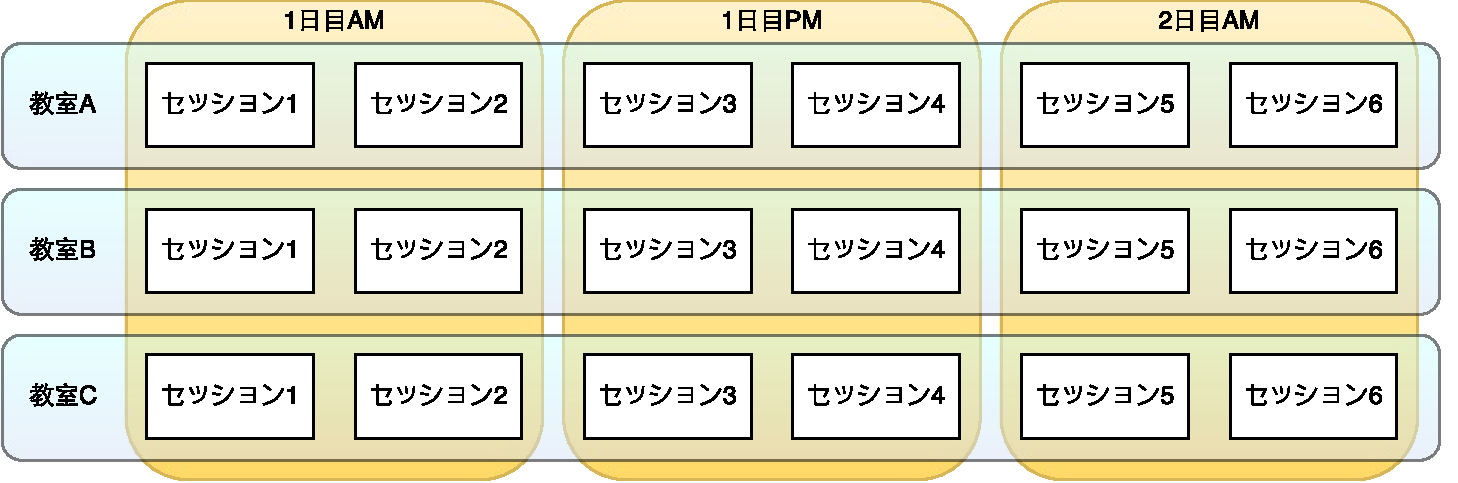
\includegraphics[width=9cm,height=4cm]{Session.pdf}
   \end{center}
}

\frame{
  \frametitle{最適化モデルの内容(一部)}
  \begin{beamerboxesrounded}[shadow=false]
    {絶対制約}
    \begin{itemize}
    \item 学生は、自分自身と担当教員が共に参加可能なセッションで発表する
    \item 研究室が同じ学生は教室をまたいで\\同時刻のセッションで発表することはない
    \end{itemize}
  \end{beamerboxesrounded}
  %
  \begin{beamerboxesrounded}[shadow=false]
    {考慮制約}
    \begin{itemize}
    \item 同時刻に行われるセッションの発表人数の\\最大と最小の差は$1$以下とするのが望ましい
    \item 各研究室はすべての時間帯で発表するのが\\望ましい
    \end{itemize}
  \end{beamerboxesrounded}  
}

\frame{
  \frametitle{現在の最適化モデルの問題点($1/3$)}
  %
  \begin{itemize}
  \item 求解時間が長く、最適解を求め切れていない\\ケースがある
    \begin{itemize}
      \item 各セッションの発表人数の上限に奇数が増えると\\求解時間が急激に伸びる
    \end{itemize}
  \end{itemize}
   \begin{center}
      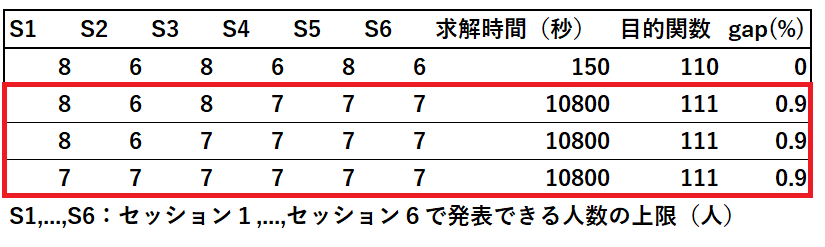
\includegraphics[width=10cm,height=4.5cm,]{gap.PNG}
    \end{center}
}


\frame{
  \frametitle{現在の最適化モデルの問題点($2/3$)}
  \begin{itemize}
  \item 追加したい要件がある(ある教員の要望) 
  \end{itemize}
  \begin{itembox}[l]{追加したい要件}
    研究内容が近い研究室の教員が、お互いの研究室の\\発表を聞けるようにしたい
  \end{itembox}
  %
  \begin{itemize}
  \item 現在のモデルは発表順序を考慮していない
    \begin{itemize}
    \item 発表日程、教室、セッションのみを考慮
    \end{itemize}
  \end{itemize}
  %
}

\frame{
  \frametitle{現在の最適化モデルの問題点($3/3$)}
  %
  \begin{itemize}
  \item 研究室Aの教員が研究室Bの学生の発表を\\   聞きたいときに、発表順序を考慮すると\\教室の移動が可能な場合がある
  \end{itemize}
  \begin{figure}[tpb]		
    \begin{center}	
      \includegraphics[scale=0.5]<1>{BeforeOrder.PNG}
      \includegraphics[scale=0.5]<2>{AfterOrder.PNG}
    \end{center}
  \end{figure}
  %
}

\frame{
  \frametitle{インターフェースの機能($1/2$)}
  %
  \begin{itemize}
  \item 利用教室や発表人数の上限などのデータを入力
  \end{itemize}
  \begin{center}
    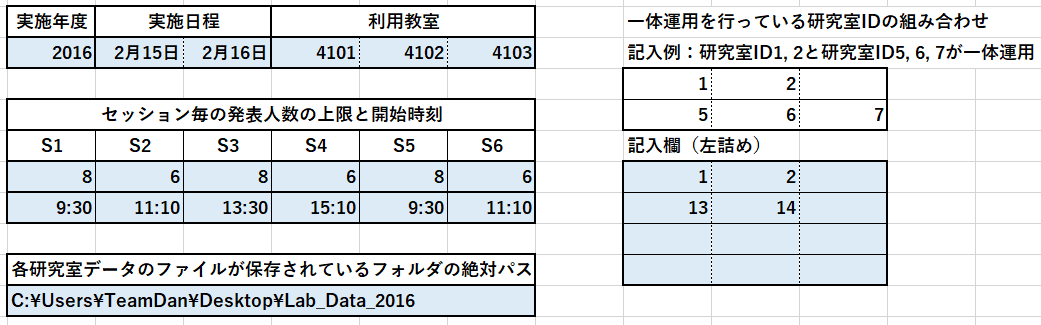
\includegraphics[width=10cm,height=4.5cm,]{InterFace2.PNG}
  \end{center}
  %
}


\frame{
  \frametitle{インターフェースの機能($2/2$)}
  %
  \begin{itemize}
  \item 各研究室の情報(図参照)を元に最適化計算用の\\データファイルを作成
  \end{itemize}
  \begin{center}
    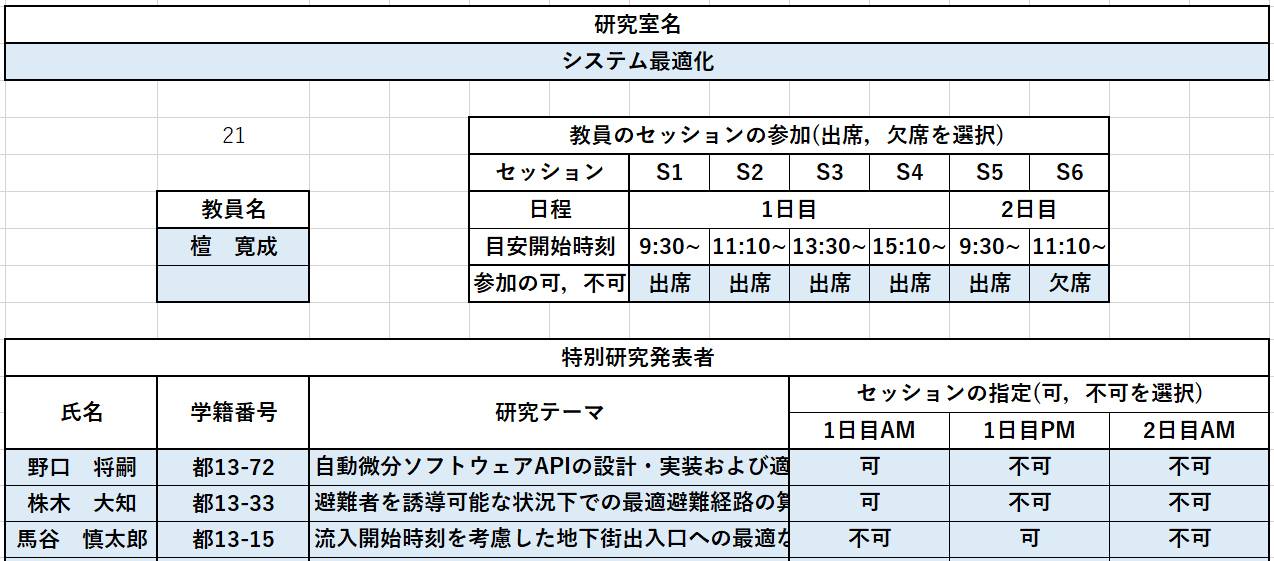
\includegraphics[width=9cm,height=4.5cm]{LabData.PNG}
  \end{center}
  \begin{itemize}
  \item 最適化ソルバを用いて求解
  \item 求解結果からスケジュール一覧表を作成
  \end{itemize}
  %
}


\frame{
  \frametitle{現在のインターフェースの問題点}
  %
  \begin{itemize}
  \item インターフェース実行までに多くの準備が必要
    \begin{itemize}
    \item モデルファイルやバッチファイルなど
    \end{itemize}
  \item 利用環境が変わるたび設定が必要
    \begin{itemize}
    \item バッチファイルの書き換えや絶対パスの変更など
    \end{itemize}
  \end{itemize}
  \begin{screen}
   {\scriptsize
     \verbatimtabinput{FileConvert.bat}
     }
  \end{screen}
  \begin{itemize}
  \item 手間を要し、インターフェースの保守性が\\損なわれる可能性がある
  \end{itemize}
}


\frame{
  \frametitle{まとめと今後の課題}
  %
  \begin{beamerboxesrounded}[shadow=false]
    {まとめ}
    \begin{itemize}
    \item 最適化モデルについて
      \begin{itemize}
      \item 求解時間の短縮
      \item 追加したい要件の実現
      \end{itemize}
    \item インターフェースについて
      \begin{itemize} 
      \item 利便性の向上
      \end{itemize}
    \end{itemize}
  \end{beamerboxesrounded}
  %
  \begin{beamerboxesrounded}[shadow=false]
    {今後の課題}
    \begin{itemize}
    \item 最適化モデルの再検討
    \item アンケートを実施し、追加・変更したい部分の調査
    \item Excel以外でのインターフェースの開発
    \end{itemize}
  \end{beamerboxesrounded}
}


\appendix
\backupbegin

\frame{
  \frametitle{スケジュール作成問題の定式化 ($1/3$)}
  \begin{beamerboxesrounded}[shadow=false]{絶対制約 ($1/2$)}
    \begin{itemize}
    \item 全学生が $1$ 回ずつ発表する
    \item 学生は自分自身と研究室の教員が共に\\参加可能なセッションで発表する
    \item 各研究室は複数のセッションで発表する
    \item 研究室が同じ学生は教室をまたいで同時刻の\\セッションで発表しない
    \item 学生個人の発表と,指定された研究室に所属する\\学生の発表が対応する
    \item 一体運用を行う研究室は同じセッションにて\\発表する
    \end{itemize}
  \end{beamerboxesrounded}
  %
}

\frame{
  \frametitle{スケジュール作成問題の定式化 ($2/3$)}
  \begin{beamerboxesrounded}[shadow=false]{絶対制約 ($2/2$)}
    \begin{itemize}
    \item 各セッションの発表人数の計算
    \item 各セッションの発表者数は上限を超えない
    \item 研究室の時間帯毎の発表者数の計算
    \item 全セッションで教員が司会をする
    \item 研究室での発表がある場合,(その研究室の)\\教員が司会をすることがある
    \item 各教員が司会をするのは $1$ 度までとする
    \end{itemize}
  \end{beamerboxesrounded}
  %
}

\frame{
  \frametitle{スケジュール作成問題の定式化 ($3/3$)}
  \begin{beamerboxesrounded}[shadow=false]{考慮制約}
    \begin{itemize}
    \item 同時刻に行われているセッションにおいて\\発表人数の最大と最小の差は $1$ 以下とするのが\\望ましい
    \item 各研究室は全ての時間帯で発表するのが\\望ましい
    \item 各研究室の中で,時間帯毎の発表者数の差は\\少ない状態が望ましい
    \item 同じセッションで発表するのが望ましい学生の\\組合せをできるだけ成立させる
    \end{itemize}
  \end{beamerboxesrounded}
  %
}

\backupend


\end{document}
%%%%% End of file %%%%%
